\documentclass[
  %%%%%%%%%%%%%%%%%%%%%%%%%%%%%%%%%%%%%%%
  % HIF people may want to uncomment this
%  hif,
  %%%%%%%%%%%%%%%%%%%%%%%%%%%%%%%%%%%%%%%
  %
  %uncomment this to suppress the Dresden Concept logo
%  noddclogo,
  %
  %uncomment this if you don't like the navigation buttons (prev/next slide, full-screen)
%  nonavigation,
  %
  %uncomment this if you want the title page and/or part page text to be aligned flushleft
%  titlepageflushleft,
%  partpageflushleft,
  %
  %for wide-screen (16:9) projectors enable this
  aspectratio=169,
  %
  % normal font size
  10pt
]{beamer}

%%%%%%%%%%%%%%%%%%%
% language settings
%%%%%%%%%%%%%%%%%%%
\usepackage[ngerman,english]{babel} % primary: US-English
%\usepackage[english,ngerman]{babel} % primary: German

% font settings; change as needed
\usepackage[T1]{fontenc}
\usepackage{lmodern}
\usefonttheme[onlymath]{serif}

% add your packages here
\usepackage{fancyvrb}
\usepackage{tikz}
\usepackage{amsmath}

\usepackage{xcolor}
\definecolor{shadecolor}{RGB}{200,200,200}
\newcommand{\terminal}[1]{\par\noindent\colorbox{shadecolor}
{\parbox{\dimexpr\textwidth-2\fboxsep\relax}{\texttt{#1}}}}

\usepackage[normalem]{ulem} % \uline for underlining main author
\ExplSyntaxOn
\pdfstringdefDisableCommands{\def\uline#1{\str_uppercase:f{#1}}}
\ExplSyntaxOff

% look for the hzdr theme in the current directory too
\makeatletter\def\input@path{{beamerthemehzdr/}}\makeatother
\usetheme{hzdr}

%%%%%%%%%%%%%%%%%%%%%%%%%%%%%%%%%%%%%%%%%%%%%%%%%%%%%%%%%%%%%%%%%%%%%%%%%%%%%%
%    title, author, date, institute, additional logos
%%%%%%%%%%%%%%%%%%%%%%%%%%%%%%%%%%%%%%%%%%%%%%%%%%%%%%%%%%%%%%%%%%%%%%%%%%%%%%

%\title[short version, used in the footline]{long version in the title page}
\title[]{Hands-on training for PIConGPU users}
\subtitle{getting started with PIConGPU on LUMI} % may be left empty, of course

%\author[short version of authors (not used, currently)]{long version in the title page}
\author[R. Pausch, et al.]{\uline{Richard Pausch}\inst{1}, Sergey Bastrakov\inst{1}, Michael Bussmann\inst{1,2}, Finn-Ole Carstens\inst{1}, Alexander Debus\inst{1}, Fabia Dietrich\inst{1}, Sergey Ermakov\inst{1,3}, Julian Lenz\inst{1,2}, Brian Marre\inst{1}, Tapish Narwal\inst{1,2}, Pavel Ordyna\inst{1}, Klaus Steiniger\inst{1,2}, Jessica Tiebel\inst{1}, René Widera\inst{1}}

%\date[short date]{long date}
\date[2024-10-25]{{2024-10-25}} % texdoc datetime2

\institute[
  %short version of main authors' institute, used in the footline (not used, currently)
]{%
  %long version, used in the title page
    \inst{1}Helmholtz-Zentrum Dresden -- Rossendorf \\[1ex]
    \inst{2}CASUS - Center for Advanced Systems Understanding \\[1ex]%
    \inst{3}ETH Zürich
}

%%%%%%%%%%%%%%%%%%
% partner logos
%%%%%%%%%%%%%%%%%%

%every invocation of \partnerlogo{...} adds yet another logo to the
%right of already inserted partner logos; logos are automatically scaled
\partnerlogo{
\includegraphics{Plasma-PEPSC-Logo_black.png}}
%\partnerlogo{\fboxsep=1em\colorbox{gray!40}{Logo 2}}

%%%%%%%%%%%%%%%%%%%%%%%%%%%%%%%%%%%%%%%%%%%%%%%%%%%%%%%%%%%%%%%%%%%%%%%%%%%%%%

%hzdr colours used for various text highlights; see manual (texdoc beamer),
%for further possibilities
                                                 %colour will be used in:
\setbeamercolor{alerted text}{fg=hzdr-orange-60} %\alert{text to be highlighted},
                                                 %\begin{alertenv} ... \end{alertenv}
                                                 %\begin{alertblock}{block title (highlighted)}
                                                 %  ...
                                                 %\end{alertblock}

\setbeamercolor{example text}{fg=hzdr-blue-60} %\begin{exampleblock}{block title (highlighted)}
                                               %  ...
                                               %\end{exampleblock}
\hypersetup{%
  breaklinks,colorlinks,
  %pdfpagemode=FullScreen,
  %pdfhighlight=/P,
  linkcolor=hzdr-blue,
  linkcolor=hzdr-blue,
  anchorcolor=hzdr-blue,
  citecolor=hzdr-blue,
  filecolor=hzdr-blue,
  menucolor=hzdr-blue,
  runcolor=hzdr-blue,
  urlcolor=hzdr-blue
}

% color definitions
\definecolor{hz-blue}{RGB}{0,90,160}
\definecolor{hz-dark-blue}{RGB}{10,45,110}
\definecolor{hz-green}{RGB}{140,180,35}
\definecolor{hz-gray}{RGB}{90,105,110}

%%%%%%%%%%%%%%%%%%%%%%%%%%%%%%%%%%%%%%%%%%%%%%%%%%%%%%%%%%%%%%%%%%%%%%%%%%%%%%
%                            document starts here                            %
%%%%%%%%%%%%%%%%%%%%%%%%%%%%%%%%%%%%%%%%%%%%%%%%%%%%%%%%%%%%%%%%%%%%%%%%%%%%%%
\begin{document}
\frame{\titlepage}

\begin{frame}[t,fragile]{Introduction}

\Large  \textbf{What will we do today? }
  {\Large
  \begin{enumerate}
      \item check your access to LUMI
      \item setup and run first PIConGPU simulation
      \item data analysis of simulation using openPMD and Jupyter
      \item dive deeper into how to setup a PIConGPU simulation
      \item time for questions
      \item start another project on your own
  \end{enumerate}
}
  
\end{frame}

\part{Check LUMI access}
\frame{\partpage}

\begin{frame}{Accessing LUMI}{Checking you are part of the workshop project}
\begin{itemize}
    \item go to: \url{https://my.lumi-supercomputer.eu/}
    \item login with your credentials
    \item go to projects and check whether you have access to\\ 
    \textbf{ENCCS training (EHPC-DEV-2024D09-003)}\\
    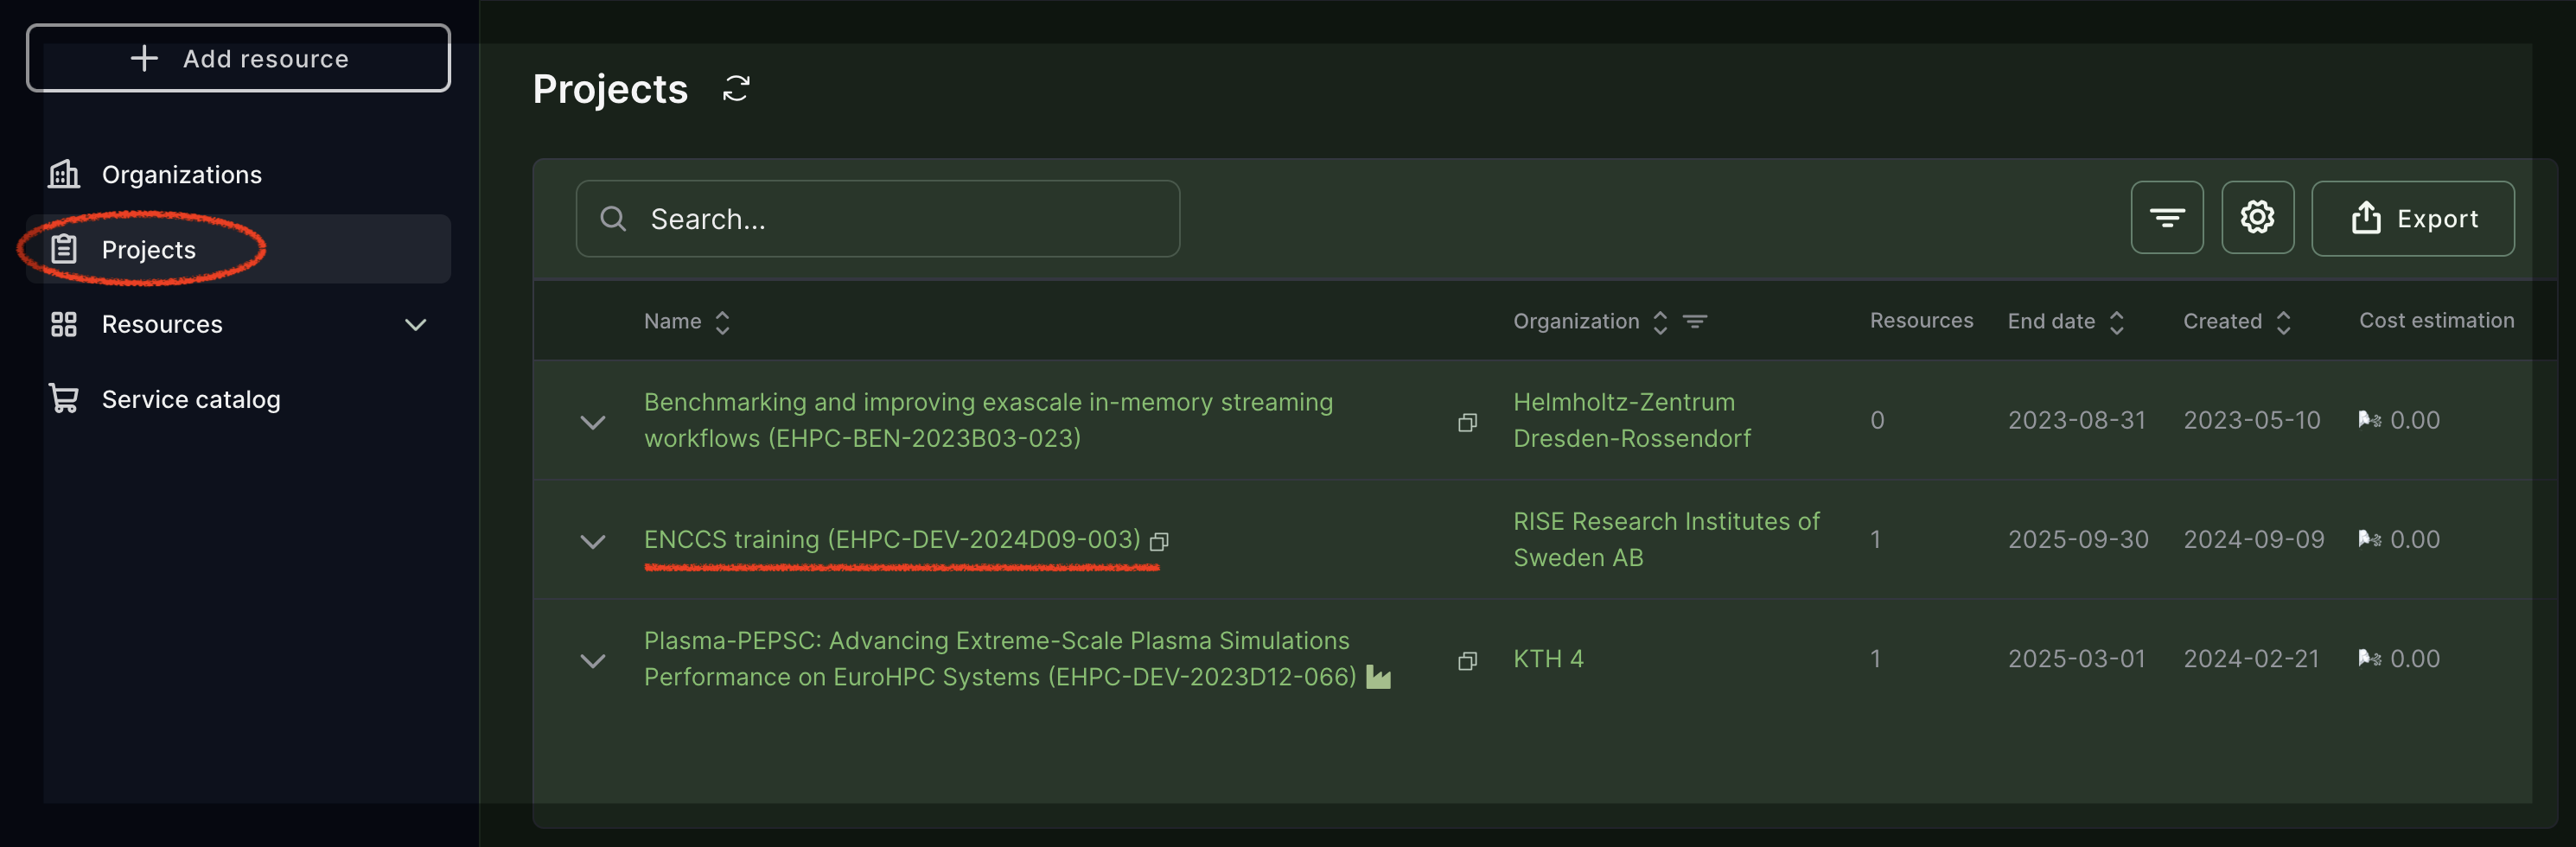
\includegraphics[width=0.8\textwidth]{images/LUMI_projects.png}
\end{itemize}

\end{frame}



\begin{frame}[t,fragile]{Accessing LUMI}{Setting up an SSH key pair}

\begin{itemize}
    \item create a (LUMI specific) key pair:\\
    \terminal{ssh-keygen -t ed25519 -f /home/username/.ssh/id\_juwels\_ed25519}
    \item now you should have:
        \begin{itemize}
            \item your private key: \texttt{id\_lumi\_ed25519}
            \item and your public key: \texttt{id\_lumi\_ed25519.pub}
        \end{itemize}
    \item go to: \url{https://mms.myaccessid.org/profile/}\\
    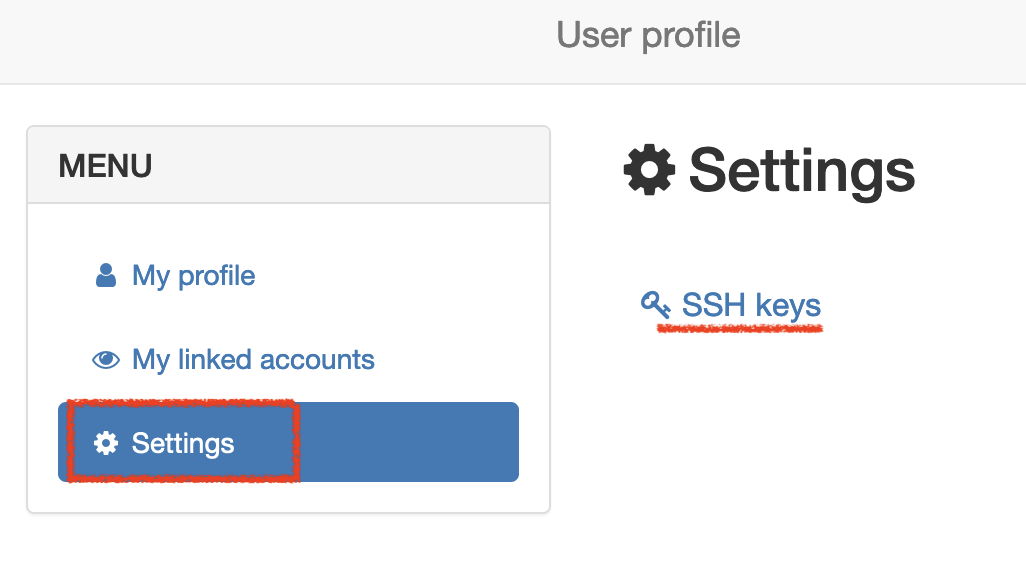
\includegraphics[width=0.4\textwidth]{images/LUMI_key_registration.png}
    \item upload your \textbf{public} key
\end{itemize}

\end{frame}


\begin{frame}[t,fragile]{Accessing LUMI}{ssh into LUMI}

\begin{itemize}
    \item execute: \terminal{ssh -i ~/.ssh/id\_lumi\_ed25519 your\_username@lumi.csc.fi}
    \item you should see:\newline
    
\includegraphics[width=0.7\textwidth]{images/LUMI_terminal.png}
\end{itemize}

\end{frame}


\begin{frame}[t,fragile]{Accessing LUMI}{your workshop project}

\begin{itemize}
    \item check which projects you have access to: 
    \terminal{lumi-allocations }
    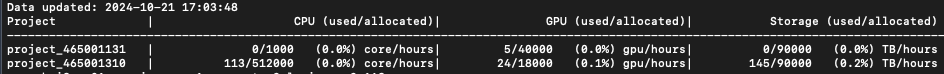
\includegraphics[width=0.8\textwidth]{images/LUMI_projects2.png}
    \item compare to: \newline
    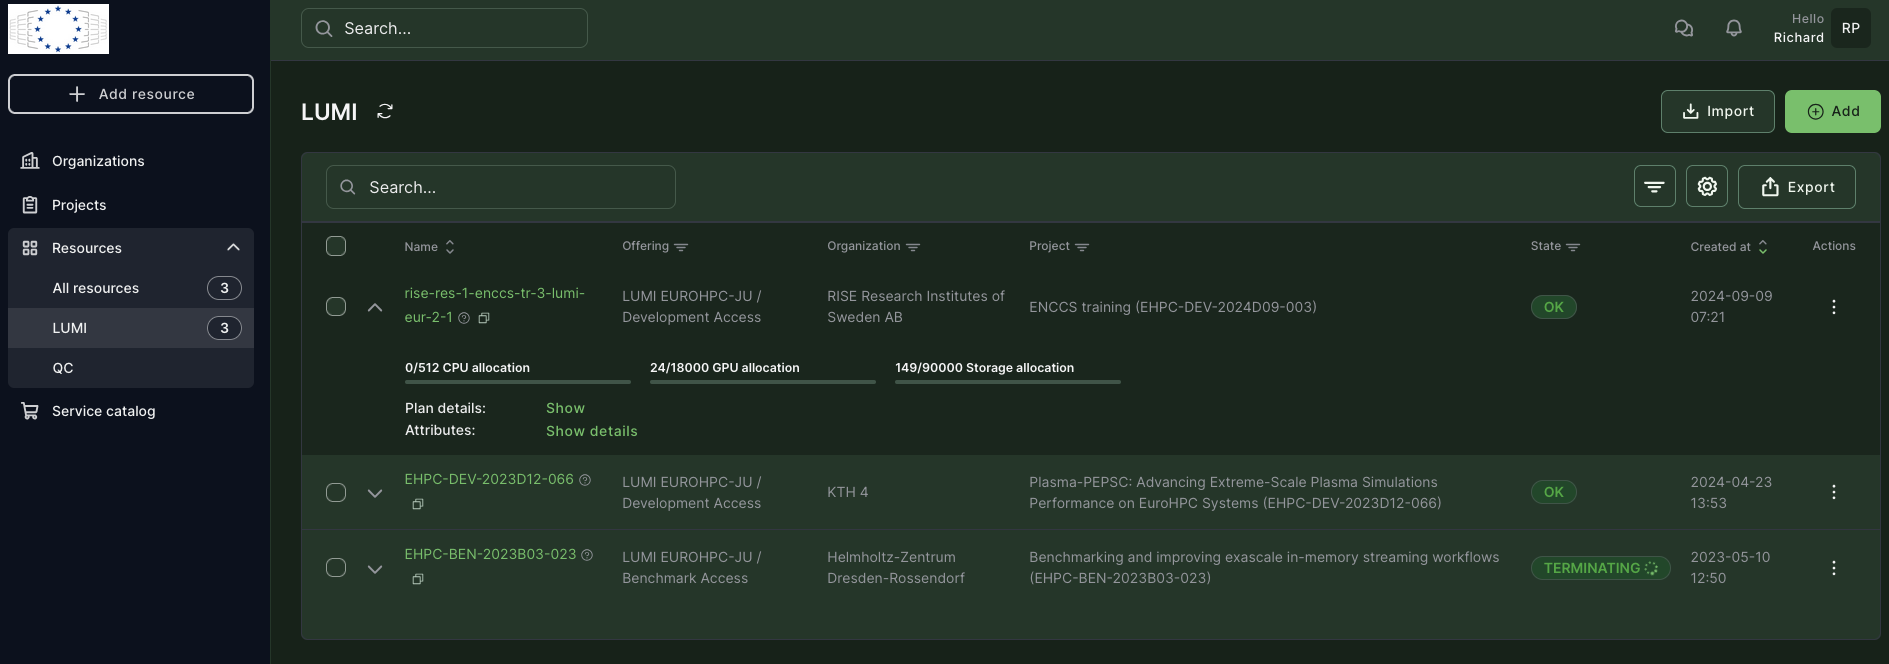
\includegraphics[width=0.8\textwidth]{images/LUMI_projects3.png}
\end{itemize}

\end{frame}

\begin{frame}[t,fragile]{Accessing LUMI}{alternative access via browser}

\begin{itemize}
    \item LUMI offers a web interface \begin{center}\textbf{\url{www.lumi.csc.fi}}\end{center}
    \item login with you credentials  
    \item select compute node shell
    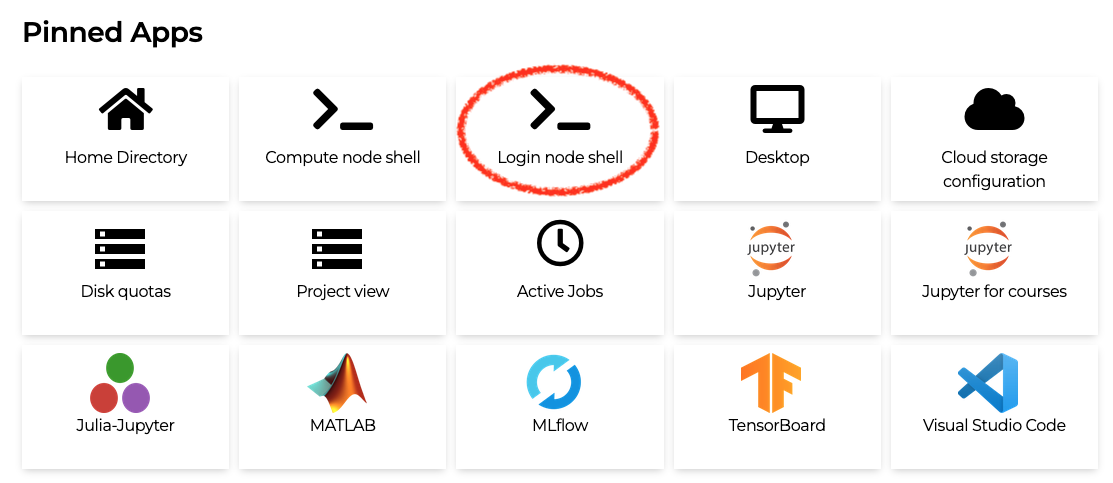
\includegraphics[width=0.7\textwidth]{images/LUMI_web_shell2.png}
\end{itemize}

\end{frame}



\begin{frame}[t,fragile]{Accessing LUMI}{creating your working directories}

\begin{itemize}
    \item we are working with \begin{center}\textbf{\texttt{project\_465001310}}\end{center}
    \item project directory \begin{center}\textbf{\texttt{/projappl/project\_465001310}}\end{center}
    \item please create a directory there \terminal{cd /projappl/project\_465001310 \newline mkdir \$(whoami)}
    \item simulation directory \begin{center}\textbf{\texttt{/scratch/project\_465001310}}\end{center}
    \item please create a directory there \terminal{cd /scratch/project\_465001310 \newline mkdir \$(whoami)}    
\end{itemize}

\end{frame}






\part{First PIConGPU simulation}
\frame{\partpage}

\begin{frame}[t,fragile]{Setting up PIConGPU (on LUMI)}{There is a manual!}
\begin{center}
    {\Large
    \vspace{1\baselineskip}
    \textcolor{hz-blue}{\textbf{   \url{https://picongpu.readthedocs.io}   }}\\
    \vspace{1\baselineskip}
    \textbf{is your first source of help!}\\
    \vspace{1\baselineskip}}
    {\large The steps we follow now are similar to the `PIConGPU in 5 Minutes on Hemera' tutorial there.}
\end{center}

\end{frame}




\begin{frame}[t,fragile]{Performing PIConGPU simulations}{The general workflow}
\begin{enumerate}
    \item \textbf{Get PIConGPU }\\
        \terminal{\$ git clone  https://github.com/ComputationalRadiationPhysics/picongpu.git}
    \item \textbf{Prepare and load environment}\\
        \terminal{\$ source picongpu.profile}
    \item \textbf{Create simulation setup}\\
        \terminal{\$ pic-create \$PIC\_EXAMPLES/LaserWakefield myLWFA}
    \item \textbf{Adjust setup parameters}\\
        \terminal{\$ vim simulation.param}
    \item \textbf{Compile setup}\\
        \terminal{\$ pic-build}
        %\terminal{\$ pic-build 2>err.txt; sleep 2s; rm -r .build}
    \item \textbf{Run setup (submit to batch system)}\\
        \terminal{\$ tbg -s -t -c etc/picongpu/*.cfg mySimOutputDirectory}
    \item \textbf{Analyze results}\\
        \terminal{\$ jupyter-lab}
%    \item \textbf{}\\
%        \terminal{\$ }
\end{enumerate}
\end{frame}




\begin{frame}[t,fragile]{Setting up PIConGPU on LUMI}{(1) get the source code}

\begin{itemize}
    \item download the PIConGPU source code:
    \begin{itemize}
        \item into project directory
        \terminal{\# option 1 \newline 
        cd /projappl/project\_465001310/\$(whoami)}
        \item or in home directory
        \terminal{\# option 2 \newline
        cd \$HOME/ \newline
        mkdir src \newline
        cd src}
    \end{itemize}
    \item get source code
    \terminal{git clone https://github.com/ComputationalRadiationPhysics/picongpu.git}
\end{itemize}

\end{frame}


\begin{frame}[t,fragile]{Setting up PIConGPU on LUMI}{(2) prepare and load environment}

\begin{itemize}
    \item copy default setup file:
    \terminal{cp picongpu/etc/picongpu/lumi-eurohpc/lumi-G\_hipcc\_picongpu.profile.example /projappl/project\_465001310/\$(whoami)/lumi-G\_hipcc\_picongpu.profile}

    \item either use your editor of choice in the terminal (vim, emacs, nano) or use the web interface 
    \item adjust the following lines:
    \begin{enumerate}
        \item[8] \texttt{export MY\_MAILNOTIFY="ALL"}
        \item[9] \texttt{export MY\_MAIL="your.mail@server.gov"}
        \item[16] \texttt{export PROJID=project\_465001310}
        \item[17] \texttt{export PROJECT\_DIR=/projappl/\$PROJID/}
        \item[18] \texttt{export SCRATCH=/scratch/\$PROJID/}
        \item[27] \texttt{export EDITOR="emacs -nw"}
        \item[72] \texttt{export PIC\_LIBS=\$PROJECT\_DIR/workshop\_software/local}
        \item[81] \texttt{export PICSRC=\$PROJECT\_DIR/\$(whoami)/picongpu}
    \end{enumerate}
    
\end{itemize}

\end{frame}




\begin{frame}[t,fragile]{Setting up PIConGPU on LUMI}{(3) Create simulation setup}
    \terminal{%
        mkdir -p picInputs\\
        cd picInputs\\
        pic-create LaserWakefield LWFA
    }
\begin{itemize}
    \item ...
    \item peek into \texttt{include/picongpu/param}:\\
        \terminal{\$ ls -l include/picongpu/param}\\
        $\Rightarrow$ The \texttt{*.param} files largely define the simulation setup
\end{itemize}

\end{frame}



\begin{frame}[t,fragile]{Setting up PIConGPU on LUMI}{(4.1) Adjust setup parameters}

\begin{itemize}
    \item for now we will not go into details
    \item just to follow the workflow, we will adjust \textbf{one compile-time} parameter
    \item compile-time parameters are in \texttt{include/picongpu/param}
    \item let's see where the parameter files are:
    \terminal{cd LWFA/include/picongpu/param \\
    ls -l}
    \item let's edit the laser configuration
    \terminal{vim incidentField.param}
    \begin{enumerate}
        \item[66] change $a_0$ from $8.0$ to $5.0$ 
    \end{enumerate}

\end{itemize}

\end{frame}




\begin{frame}[t,fragile]{Setting up PIConGPU on LUMI}{(4.2) Adjust setup parameters}

\begin{itemize}
    \item just to follow the workflow, we will adjust \textbf{one run-time} parameter
    \item run-time parameters are in \texttt{etc/picongpu/*.cfg}
    \item let's see where the parameter files are:
    \terminal{cd - \\ cd LWFA/etc/picongpu/ \\
    ls -l}
    \item let's edit the \texttt{4.cfg}
    \terminal{vim 4.cfg}
    \begin{enumerate}
        \item[68] remove checkpointing and add mapped memory strategy
    \end{enumerate}
\end{itemize}


\begin{verbatim}
TBG_openPMD="--openPMD.period 100 \\
             --openPMD.file simData \\
             --openPMD.ext bp \\
             --openPMD.dataPreparationStrategy mappedMemory"
\end{verbatim}



\end{frame}





\begin{frame}[t,fragile]{Setting up PIConGPU on LUMI}{(5) compile setup}

\begin{itemize}
    \item go back to the root of your LWFA example 
    \terminal{cd -}
    \item compile your setup
    \terminal{pic-build }
    \item better: 
    \terminal{pic-build  -f 2> err.txt}
    \begin{itemize}
        \item Allows to read errors in \texttt{err.txt} (after compiling)
        \item Using option \texttt{-f} ensures we do not use cached \texttt{*.param} files but the original ones during compile.
            Accidentally using cached files is a common source of errors.
        \item \texttt{-c ...} fixes a current issue with CMake

    \end{itemize}
    \end{itemize}
\end{frame}



\begin{frame}[t,fragile]{Setting up PIConGPU on LUMI}{You can spend compile time to rethink your parameter choices\\(or check the latest xkcd...)}
\begin{center}
    \Large
    \terminal{pic-build -f 2> err.txt}\\
    \vspace{\baselineskip}
    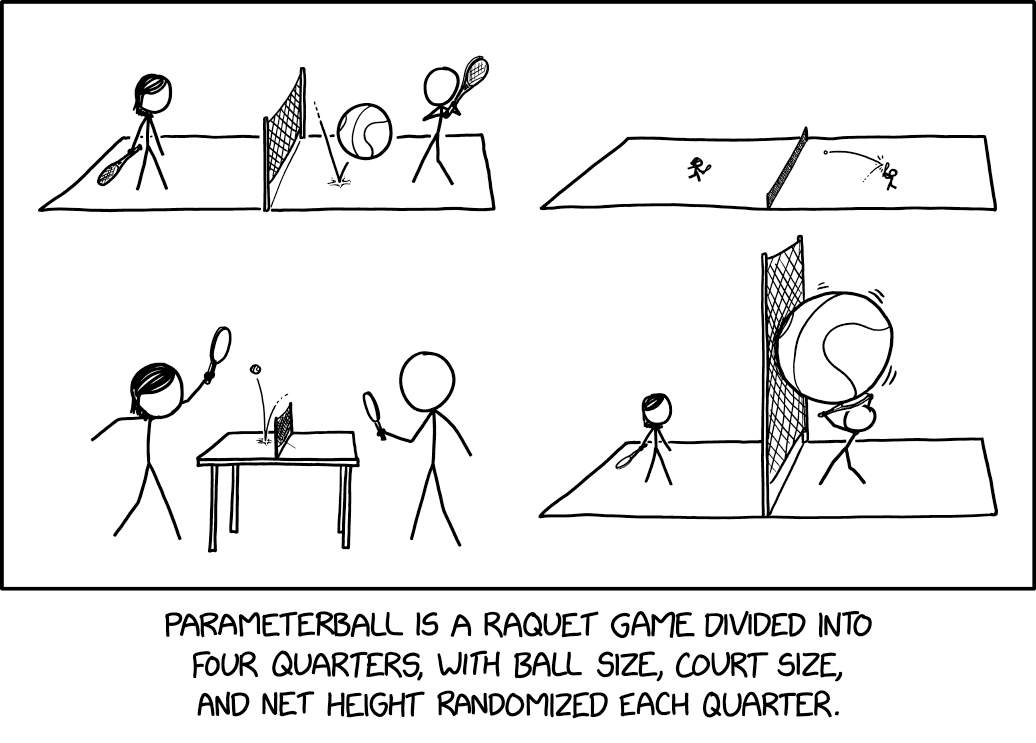
\includegraphics[width=0.45\textwidth]{images/parameterball_2x_xkcd-2852.png}
\end{center}
\end{frame}



\begin{frame}[t,fragile]{Setting up PIConGPU on LUMI}{We have a reservation}
\begin{itemize}
    \item in order to get your simulation to start, please use today's reservation
    \item the reservation is called:
    {\Large
    \begin{center}
        \texttt{ENCCS\_day3}
    \end{center}
    }
    \item adjust or \texttt{tbg} template file
    \terminal{vim etc/picongpu/lumi-eurohpc/standard-g.tpl}
    replace line 25: \\
    \begin{verbatim}
    #SBATCH --partition=!TBG_queue
    \end{verbatim}
    with:
    \begin{verbatim}    
    #SBATCH --reservation=ENCCS_day3
    #SBATCH --exclusive
    \end{verbatim}    
\end{itemize}
\end{frame}


\begin{frame}[t,fragile]{Setting up PIConGPU on LUMI}{(6) Run setup}
\begin{itemize}
    \item submit job using \texttt{tbg} (assuming you changed the \texttt{standard-g.tpl})
    \terminal{%
        tbg -s -t -c etc/picongpu/4.cfg \$SCRATCH/\$(whoami)/01\_LWFA
    }
    \item \texttt{tbg} stand for Template Batch Generator and is our abstraction for setups for various clusters
    \item it sets a submit command via \texttt{-s} (default on LUMI: \texttt{sbatch})
    \item it uses a template via \texttt{-t} (default on LUMI: \texttt{standard-g.tpl})
    \item it uses a setup configuration 
    \item does your job run?
        \terminal{%
            squeue -u \$USER\\
            scontrol show jobid \textit{<Your job's id>}
        }
\end{itemize}
\end{frame}

\part{Data analysis with openPMD and Jupyter}
\frame{\partpage}


\begin{frame}[t,fragile]{Analysing your PIConGPU simulation}{using jupyter, openPMD-api, ...}

\begin{itemize}
    \item again use the LUMI web interface 
    \begin{center}\textbf{\url{www.lumi.csc.fi}}\end{center}
    \item login with your credentials 
    \item select Jupyter\\
    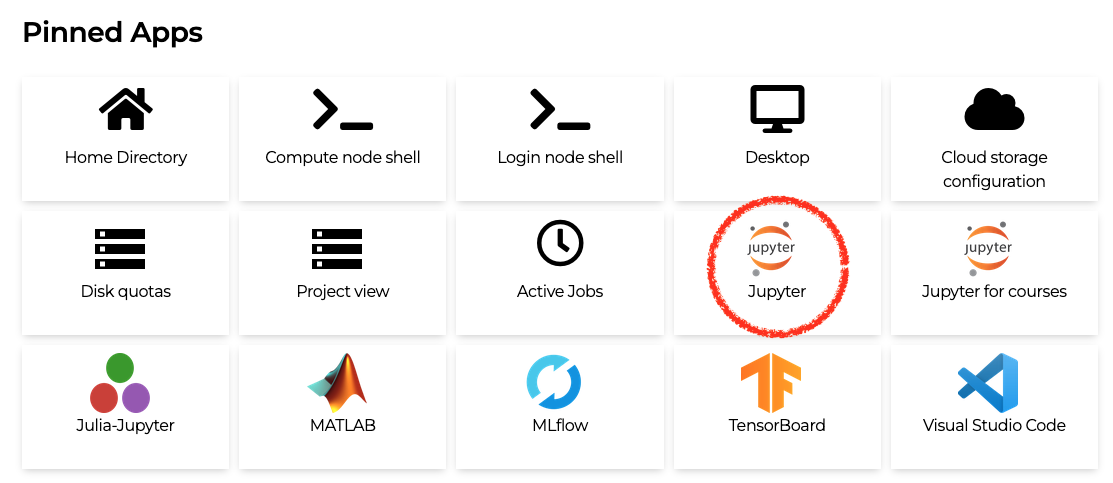
\includegraphics[width=0.7\textwidth]{images/LUMI_web_jupyter.png}
\end{itemize}

\end{frame}



\begin{frame}[t,fragile]{Analysing your PIConGPU simulation}{getting a jupyter job}

\begin{itemize}
    \item set reservation
    \item use \textbf{2 cores}
    \item use advanced setting and use prepared python environment 
    \item for now use your home directory as working directory
    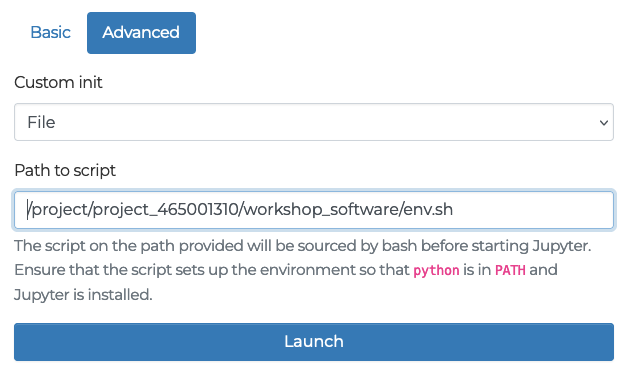
\includegraphics[width=0.6\textwidth]{images/LUMI_jupyterSetup.png}
\end{itemize}

\end{frame}


\begin{frame}[t,fragile]{Analysing your PIConGPU simulation}{run an example notebook}

\begin{itemize}
    \item copy notebook to your home directory
    \terminal{cp /projappl/project\_465001310/workshop\_software/notebooks/LWFA\_analysis.ipynb \$HOME/}
    \item change the simulation directory to your simulation path
    \item execute it
    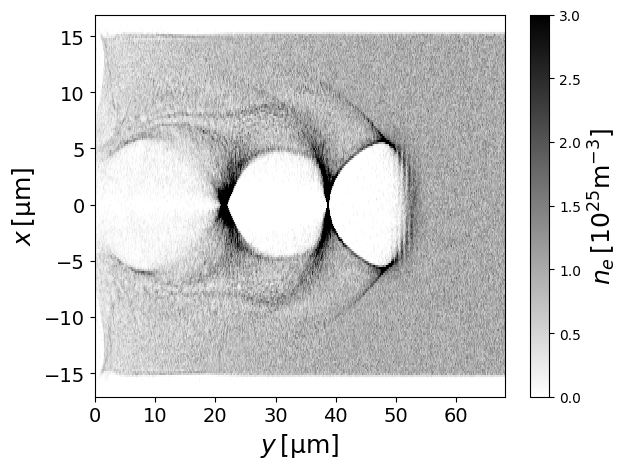
\includegraphics[width=0.35\textwidth]{images/LWFA_density.png}
    \item explore other data

\end{itemize}

\end{frame}


\part{Adjusting simulation parameters}
\frame{\partpage}


\begin{frame}[t,fragile]{PIConGPU \texttt{*.param} files}{\texttt{simulation.param}}

\begin{itemize}
    \item contains grid layout\\
    $\Delta x$, $\Delta y$, $\Delta z$, $\Delta t$
    \item reference density \\
    \texttt{BASE\_DENSITY\_SI}
    \item number of particles per cell to be initialized \\
    \texttt{TYPICAL\_PARTICLES\_PER\_CELL}

\end{itemize}

\end{frame}



\begin{frame}[t,fragile]{PIConGPU \texttt{*.param} files}{\texttt{speciesInitialization.param}}

\begin{itemize}
    \item contains a pipeline that described how macro-particles are initialized
    \begin{verbatim}
    using InitPipeline = pmacc::mp_list<
        ...>;
    \end{verbatim}
    \item particles can be created based on a density profile
    \begin{verbatim}
    CreateDensity<densityProfiles::Gaussian, 
        startPosition::Random, 
        PIC_Electrons>
    \end{verbatim} 
    \item or derived from an already existing particle distribution
    \begin{verbatim}
    Derive<PIC_Electrons, PIC_Ions>
    \end{verbatim} 
    \item particle attributes can be manipulated to set charge states, temperatures, drifts, ...

\end{itemize}

\end{frame}



\begin{frame}[t,fragile]{PIConGPU \texttt{*.param} files}{\texttt{density.param}}

\begin{itemize}
    \item LWFA contains only a Gaussian density profile
    \item let's have a look at it ...
    \item more density profiles are available, most flexible is: 
\begin{verbatim}
struct FreeFormulaFunctor
{
    HDINLINE float_X operator()(const floatD_64& position_SI, 
        const float3_64& cellSize_SI) {

        float_X s = 1.0_X - 5.0_X * math::abs(position_SI.y() - 0.0002_X);
        s *= float_X(s >= 0.0);
        return s;
    }
};
using FreeFormula = FreeFormulaImpl<FreeFormulaFunctor>;    
\end{verbatim}

\end{itemize}

\end{frame}







\begin{frame}[t,fragile]{PIConGPU \texttt{*.param} files}{\texttt{incidentField.param}}

\begin{itemize}
    \item LWFA uses Gaussian laser profile
    \item at the very end:
\begin{verbatim}
    using XMin = profiles::None;
    using XMax = profiles::None;
    using YMin = PARAM_LASERPROFILE;
    using YMax = profiles::None;
    using ZMin = profiles::None;
    using ZMax = profiles::None;    
\end{verbatim}
    \item laser definition:
\begin{verbatim}
    using GaussianProfile = profiles::GaussianPulse<GaussianPulseParam>;
\end{verbatim}    
    \item let's have a detailed look
\end{itemize}

\end{frame}




\begin{frame}[t,fragile]{Task}{run your own mini-simulation campaign}

\begin{itemize}
    \item based on your initial LWFA setup, either:
    \item simulate half and double the density and study the influence on the wakefield
    \item simulate $a_0=1.0$ and $a_0 = 0.2$ and see the effect on the wakefield
    \item play around with any other parameter you like
\end{itemize}

\end{frame}


\part{Time for your questions}
\frame{\partpage}
\begin{frame}[t,fragile]{}%Run setup}
\begin{center}
    \large
\begin{itemize}
    \item \textbf{What is ...?}
    \item \textbf{How do I do ...?}
    \item \textbf{Is it possible to ...?}\\
        Yes! (with enough time and effort ;-)
    \item \textbf{Where do I get more information on ...?}\\
        In order of precedence:\\
        \begin{itemize}
            \item The manual: \url{https://picongpu.readthedocs.io}
            \item Old issues \url{https://github.com/ComputationalRadiationPhysics/picongpu/issues?q=is%3Aissue}
            \item Open a new issue
        \end{itemize}
\end{itemize}
\end{center}
\end{frame}


\part{Starting from another examples}
\frame{\partpage}

\begin{frame}[t,fragile]{Explore other default examples}{setup your own example - we are her to help you}

\begin{itemize}
    \item \textbf{Kelvin Helmholtz instability}\\
    \texttt{KelvinHelmholtz} \\
    use \texttt{4.cfg} and add openPMD output \\
    \url{https://github.com/ComputationalRadiationPhysics/picongpu/tree/dev/share/picongpu/examples/KelvinHelmholtz}\\
    $\,$
    \item \textbf{Solid density foil target for proton acceleration}\\
    \texttt{FoilLCT} \\
    use \texttt{4.cfg} or \texttt{8.cfg} \\
    only uses 2D \\
    \url{https://github.com/ComputationalRadiationPhysics/picongpu/tree/dev/share/picongpu/examples/FoilLCT}
\end{itemize}

\end{frame}


\end{document}
